 \documentclass[12pt,a4paper]{article}
\usepackage{amsmath}
\usepackage{amssymb}
\usepackage{epstopdf}
\usepackage{inputenc}
\usepackage{graphicx}
\usepackage{titletoc} 
\usepackage{fancyhdr}   
\usepackage[a4paper,pdftex]{geometry}	
\usepackage[english]{babel}
\usepackage{xcolor} 
\usepackage{enumerate}
\usepackage{fix-cm} 
\usepackage[notlof]{tocbibind}
\usepackage{amsmath}
\usepackage{listings}
\usepackage{float}
\usepackage{enumitem}
\usepackage{xcolor}
\usepackage{listings}
\definecolor{vgreen}{RGB}{104,180,104}
\definecolor{vblue}{RGB}{49,49,255}
\definecolor{vorange}{RGB}{255,143,102}
\renewcommand\lstlistingname{Appendix}
\renewcommand\lstlistlistingname{Appendix}

\makeatletter
\newcommand*\@lbracket{[}
\newcommand*\@rbracket{]}
\newcommand*\@colon{:}
\newcommand*\colorIndex{%
	\edef\@temp{\the\lst@token}%
	\ifx\@temp\@lbracket \color{black}%
	\else\ifx\@temp\@rbracket \color{black}%
	\else\ifx\@temp\@colon \color{black}%
	\else \color{vorange}%
	\fi\fi\fi
}
\makeatother

\usepackage{trace}

\usepackage{subcaption}
\begin{document}
	\begin{titlepage}
		\begin{center}
			
\includegraphics[scale=.4]{Figures/Cover}\\
			\vspace{1cm}
			\bf{ \large {Department of Computer Science and Technology} }
		\end{center}
		
		\vspace{4cm}
		\centering
		\textbf{\Huge Machine Learning}
		\vspace{.5cm}
		
		{\Large Homework 2}

		\vspace{4cm}
		
		\textbf{\LARGE Sahand Sabour}
		
		
		
		\vspace{0.5cm}
		
		{\large 2020280401}
		
		
		\vfill
		
	\end{titlepage}

	\section{DeepWalk}
	
	\subsection{Motivation}
	\noindent 
	
	\subsection{Methodology}
	\noindent 
	
	\subsection{Experiments}
	\noindent 
	
	\subsection{Personal Opinion}
	\noindent 
	
	\newpage
	\section{(GCN)}
	
	\subsection{Motivation}
	\noindent 
	
	\subsection{Methodology}
	\noindent 
	
	\subsection{Experiments}
	\noindent 
	
	\subsection{Personal Opinion}
	\noindent 
	
	\subsection{Comparison with DeepWalk}
	\noindent 
	
	\newpage
	\section{CogDL}
	
	\subsection{Testing CogDL Models}
	
	\noindent In this assignment, we are asked to run two models on two different datasets by running the provided scripts. The first script is as follows: python scripts/train.py --task unsupervised\_node\_classification -- dataset wikipedia --model deepwalk; by running this script, we would be training and testing the DeepWalk model on the Wikipedia dataset for the task of node classification. The results of this process is provided in the figure below (Figure 1).
	\begin{figure}[H]
		\centering
		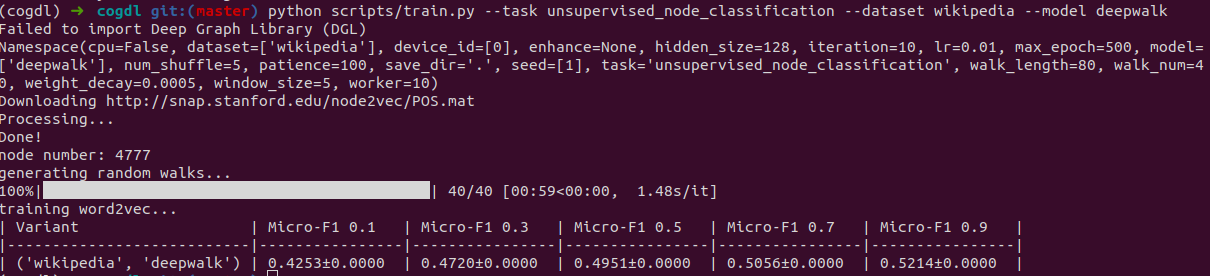
\includegraphics[width=15cm, height=5.5cm]{Figures/cmd1}
		\vspace{-0.7cm}
		\caption{Result of running the first script}
	\end{figure}

	\vspace{-0.4cm}
	\noindent Accordingly, the second script (python scripts/train.py --task node\_classification --dataset citeseer -- model gcn) analyzes the same task but for training and testing the GCN model on the citeseer dataset. The obtained results are demonstrated in the below figure (Figure 2).
	
	\begin{figure}[H]
		\centering
		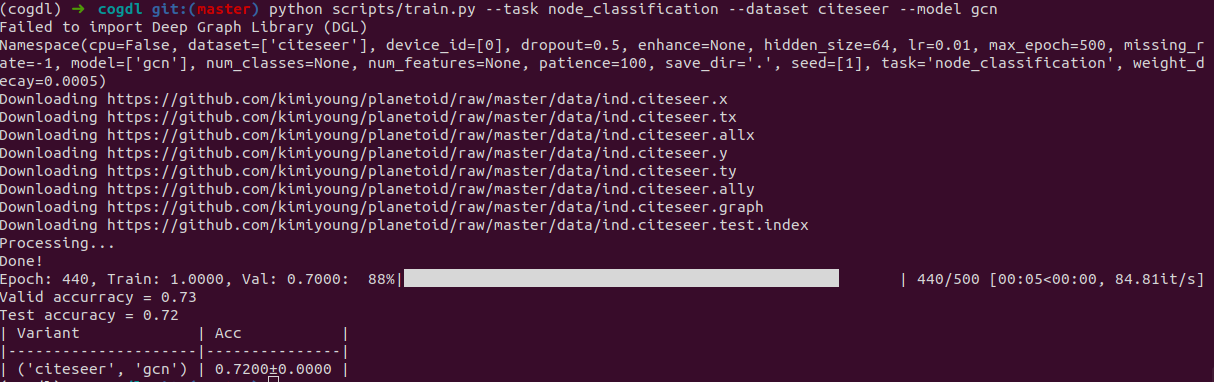
\includegraphics[width=15cm, height=6cm]{Figures/cmd2}
		\vspace{-0.7cm}
		\caption{Result of running the second script}
	\end{figure}
	
	\subsection{API Design}
	\noindent CogDL is a graph representation learning toolkit, based on PyTorch. Similar to what is demonstrated in the two scripts of the previous section, the main entry point of the model training is train.py located in the scripts folder. Initially, the arguments provided by the user are evaluated: first, it checks whether the provided arguments are valid; second, it checks whether the provided model matches the input task and dataset (based on match.yml file); third, the model implementation itself checks whether user provides all the required arguments.After the validity of the provided arguments is evaluated, CogDL checks whether the requested dataset is available offline. If this dataset has yet to be downloaded, the download script is called to download the corresponding datasets.
	
	\vspace{0.1cm}
	\noindent CogDL's API is fairly easy to use. First, setting the hyper-parameters for a specific model can be achieved by modifying the keys of 'args' variable, which is globally used in machine learning frameworks. For instance, for the task of graph classification, on the proteins dataset with the hgpsl model, we would have
	
	\vspace{-0.3cm}
	\begin{center}
		args = default\_args()\\
		args.task = 'graph\_classification'\\
		args.dataset = 'proteins'\\
		args.model = 'hgpsl'
	\end{center}

	\vspace{-0.2cm}
	\noindent In addition, the model and its dataset can be built via the following lines:
	
	\vspace{-0.2cm}
	\begin{center}
		dataset = build\_dataset(args)\\
		model = build\_model(args)\\
	\end{center}

	\vspace{-0.2cm}
	\noindent Consequently, we can create the task using the model and dataset and train it via
	
	\vspace{-0.2cm}
	\begin{center}
		task = build\_task(args, dataset=dataset, model=model)\\
		ret = task.train()\\
	\end{center}
	
	\subsection{Implementation}
	
	\noindent In this assignment, I implemented the Hierarchical Graph Pooling with Structure Learning model [1]. The pull request id for this implementation is \#80 (submitted by Sahandfer). 
	
	\subsection{Suggestions}
	\noindent There are a number of suggestions that I believe would improve the CogDL experience, both as a user and as a contributor:
	\begin{enumerate}
		\item Create a unified template for all the models for a certain tasks; this allows users to clearly differentiate between different models and provides contributors with a clear path to implement their models. 
		\item Include more information on how the evaluation results in the README.md file have been obtained. For instance, for tasks such as graph classification, there aren't any mentions of using k-folds or other arguments to make the models work on certain dataset; yet, these arguments are highly necessary.
		\item Make a list of content for the README. The current version of the README file looks rather complex, long, and hard to look through. Providing an interactive list of content would allow the users to focus on the topics of each section and find the section they are looking for much better and faster.
	\end{enumerate}
	
	\subsection{Contributions}
	
	\noindent As my contribution to this toolkit, I have made an interactive CLI to make the necessary files for a new model (check figure below).
	
	\begin{figure}[H]
		\centering
		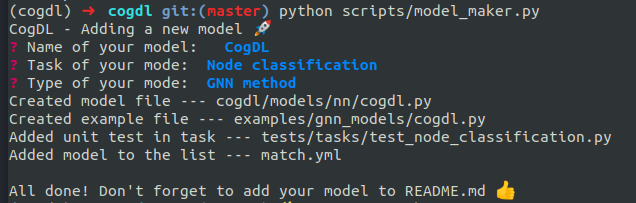
\includegraphics[width=15cm, height=6cm]{Figures/model}
		\vspace{-0.7cm}
		\caption{Model maker CLI}
	\end{figure}

	\noindent As shown in the figure, the script can be accessed by running 'python scripts/model\_maker.py'. The script then asks the user several questions to have the necessary information for creating a new file. Accordingly, the script does the following tasks based on user inputs:
	
	\begin{enumerate}
		\item Create a model file in the nn folder based on a predefined template.
		\item Create an example file in the corresponding folder of the model's type, according to a predefined template.
		\item Add the unit test for this model to the corresponding task.
		\item Add the model to the list of available models in math.yml.
		\item Remind the user to add their own model to README.md since the CLI is yet unavailable to detect the correct location to add the model. In addition, since the model is yet to be defined, its evaluation is not possible.
	\end{enumerate}

	\noindent The pull request id for this contribution is \#86 (submitted by Sahandfer).
	
	\section*{References}
	[1] Zhen Zhang et al. “Hierarchical graph pooling with structure learning”. In:arXiv(2019) arXiv:1911.05954


	
\end{document}